%学习
\chapter[学习方面]{学习方面}

\section[学分]{学分\footnotemark}
\footnotetext{因不同学制、学院、年级要求各不相同,本图仅以\textbf{2021级临床医学院临床医学系普通5年制本科}为例,依照教务处\uline{\href{https://jwch.wfmc.edu.cn/2022/0916/c5343a107934/page.htm}{《潍坊医学院本科专业人才培养方案(2021版)》}}制作,具体内容参见学生手册相关章节和教务处官网说明,如有变更恕不另行通知。}
\begin{table}[H]
    \centering
    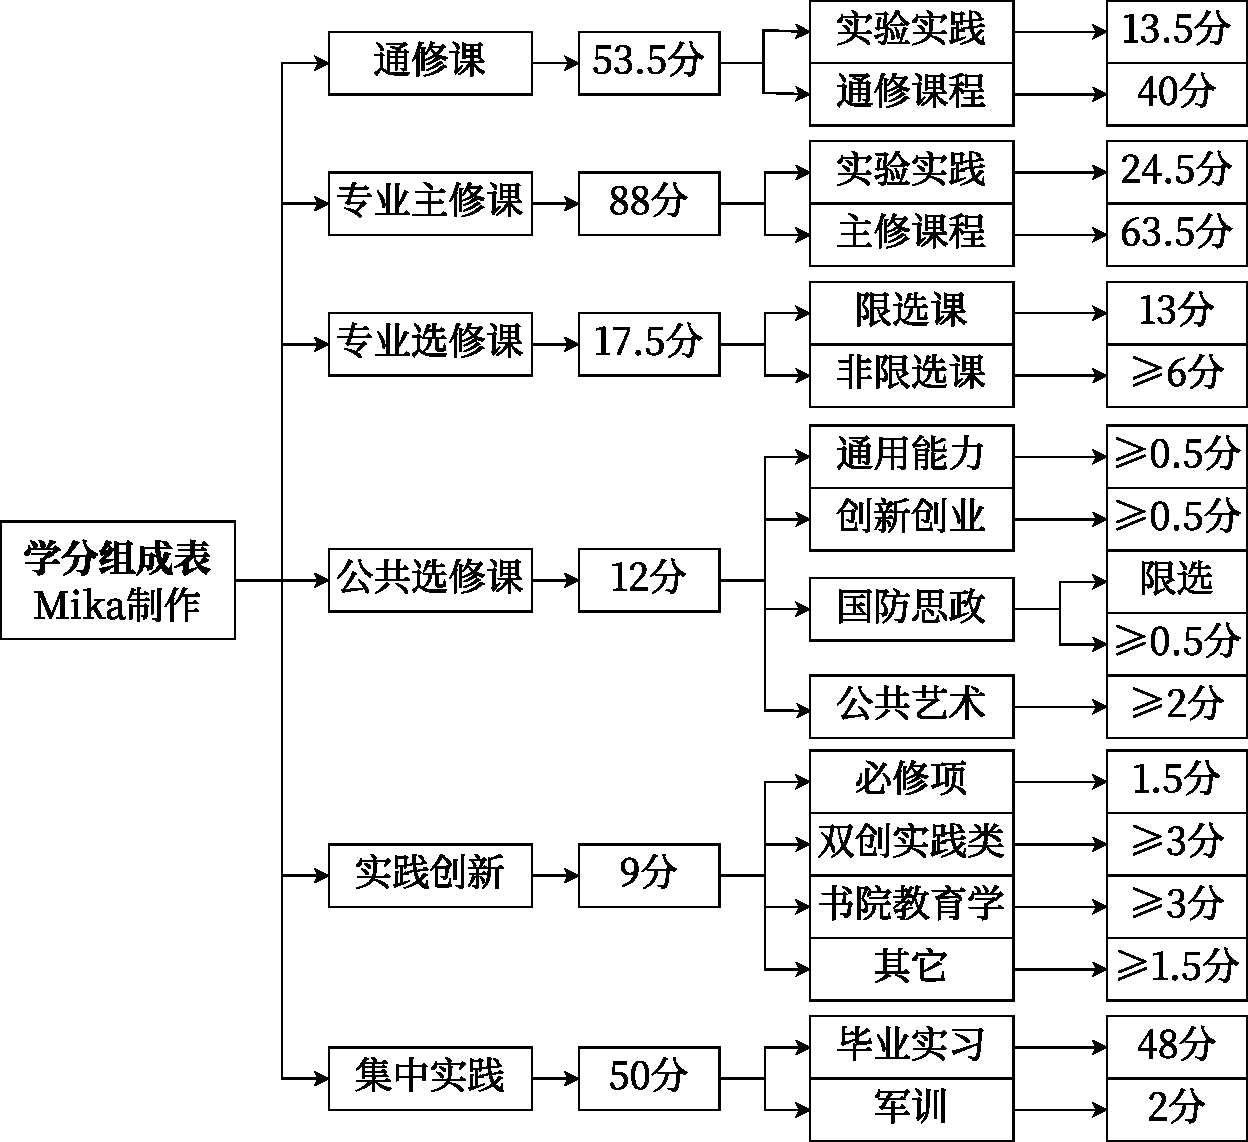
\includegraphics[width=\textwidth]{学分.pdf}
    \caption[学分组成示意图]{学分组成示意图}
    \label{score}
\end{table}

\newpage

\section[关于选修课的补充说明]{关于选修课的补充说明}
\begin{enumerate}
    \item 选修课分专业选修和公共选修两大类(详见\uline{\ref{score}}),\textbf{推荐在大一全年、大二上学期的把各类选修学分全都修满},这样就不用在后面学业愈重的情况下兼顾选修课的学习了,可以专心针对专业课程进行深入学习
    \item 专业选修课有限选和非限选之分,限选的课程无需操心,教务系统会自动选课,只需要保证非限选的课程学分达标即可
    \item 公共选修课每一类都要选至少一门,且需要满足总分,其中部分类别还有额外要求(详见\uline{\ref{score}}),国防教育类有国家限选课程(到时候看具体通知,会说的很明白的)
    \item 公共选修课有一部分是在教室上的,还有一部分是线上课程(使用“知到”app进行学习,大多数有平时分,不能突击),可以根据自己的实际情况选择\footnotemark
          \footnotetext{一般来讲线下课好过,每星期去一次教室听听课就行,结课考试也很简单;但是线上课随时都能刷课,刷完课考完试就不用每周都去听课了,根据自己的需求选择。}
    \item \textbf{\uuline{公共选修课联盟的公共选修课程不算学分、不收学费}}
\end{enumerate}

\section[自习禁止事项]{自习禁止事项}
\begin{enumerate}
    \item \textbf{禁止在教室内亲嘴、喧哗、频繁说话}
    \item \textbf{禁止在自习室内抖腿}
    \item 禁止外放音乐、视频等
    \item 禁止在大服、非本班上课常用教室占座
    \item 禁止在教室内食用气味浓的食物(例如榴梿、辣条等)
    \item 禁止长时间占用教室内电源插座,仅允许应急充电
    \item 禁止在教室以及教室旁厕所内吸烟
\end{enumerate}

\section[其他说明]{其他说明}
\begin{enumerate}
    \item \textbf{大一不参与四六级,大二才能报名四六级考试}
    \item \textbf{\uuline{转专业}\footnotemark:}
          \footnotetext{依据教务处2023年5月31日发布的\uline{\href{https://jwch.sdsmu.edu.cn/2023/0531/c2593a117986/page.htm}{《潍坊医学院2023年普通全日制本科学生转专业工作方案》}}简化,具体规定详见链接。该规定每年不一,如有变动,以教务处政策为准。}
          \begin{enumerate}
              \item 需满足以下条件:
                    \begin{enumerate}
                        \item 取得学籍的普通全日制一年级本科在校生
                        \item 未受处分、思想过硬、符合体检要求
                        \item 第一学年必修课和专业限定选修课平均成绩在本专业排名前30\%,且未挂科
                        \item 公费医学生,春季高考,第二学士学位,贯通培养学生等以特殊招生形式录取的学生;国家有相关规定或者录取前与学校有明确约定的,不得申请转专业
                    \end{enumerate}
              \item 流程:
                    \begin{enumerate}
                        \item 考试科目为思政、英语、数学,比例为1:1:1,考试时间150分钟,总分为150分
                        \item 核算学生第一学年学习成绩并公示各类数据
                        \item 8月27日开始报名
                        \item 8月31日组织考试
                        \item 9月1日-5日公示录取名单\footnotemark
                              \footnotetext{按照“分数优先,遵循志愿”的原则进行录取。}
                        \item 9月6日-7日报到
                    \end{enumerate}
          \end{enumerate}
    \item 关于奖学金\footnotemark:本校有国家奖学金、校长奖学金、校级3等级奖学金等
          \footnotetext{请注意,目前学校仅能通过本人身份开通的,已开户的,账户已激活的,无异常的,工商银行的储蓄卡发放奖学金,详情政策可咨询学校财务处。}
    \item 新生开学考试\footnotemark 的内容为高中英语、高中数学,旨在让各位同学收心
          \footnotetext{按照往年惯例,不公布具体成绩。}
    \item \textbf{关于档案填写:}开学以后需要大量填写各类表格,如果你听到“入档”这两个字时需要格外注意,入档资料具有不能涂改、不能标记、不能修正的特性,因此严禁使用修正液或修正带对其涂改(涂改修正后立即作废)。填表时务必确保各类时间填写正确、与原始档案一致。此外,建议初次填写时使用铅笔轻轻填写,待负责人确认无误后方可擦除后使用黑色中性笔或中油笔填写(入档纸张为特殊A4纸,与正常A4纸相比厚、重、滑,难以自行复印请注意)
    \item 挂科与补考、重修:因各年级、院系要求不一,详见学校下发的学生手册
    \item 关于实验课与实验服:在实验课上课时务必按要求正确洗手并佩戴头套、口罩、手套,着实验服,\textbf{\uuline{严禁任何人在任何其它地点(尤其是餐厅)着实验服}!}因在实验室中需频繁接触实验动物、微生物,\textbf{极其推荐将实验课书包与普通课书包分开}!
          \label{schoolbag}
\end{enumerate}

\section[早操与晚自习]{早操与晚自习}
\begin{enumerate}
    \item 早操时间一般为6:00~7:00,晚自习时间通常为19:00~21:00,教室22:00关闭
    \item 早操与晚自习贯穿整个大一\footnotemark,并且跑操与晚自习均有院系学生会不定时进行抽查人数是否到齐等指标,最终结果计入班级综测(详见下文\uline{\ref{class_evaluation}})的评分
          \footnotetext{按照惯例,麻醉专业无早操,只需要大一、大二早晨七点签到。}
\end{enumerate}

\section[班级综测]{班级综测}
\label{class_evaluation}
\begin{enumerate}
    \item 班级综测是用于考核各班表现的评判指标和分配见习点的依据\footnotemark,每学期计算一次,截至见习
          \footnotetext{以截至见习之前的各学期平均班级综测成绩计算班级排名,公费班级根据本年级政策进行。}
    \item 由班级平均成绩、比赛类、表彰类等类别构成,详见学生手册(各年级要求不一)
    \item 班级综测直接决定本班级同学后期学习和生活所在的医院规模、等级和生活条件(例如宿舍有无空调、暖气、洗衣机,是否提供插座,是否有早操和晚查寝\footnotemark 等),请大家务必重视
          \footnotetext{这意味着能否在外租房居住。}
\end{enumerate}
